\subsection{Medical Services Crew}

The Medical Services Crew operates follows a \textbf{sequential} task structure to plan the treatment and evacuation of injured people from the emergency site. The tasks included within the Medical Services are:

\begin{enumerate}
	\item \textbf{Task1:}
\end{enumerate}

\begin{figure}[h!]
	\centering
	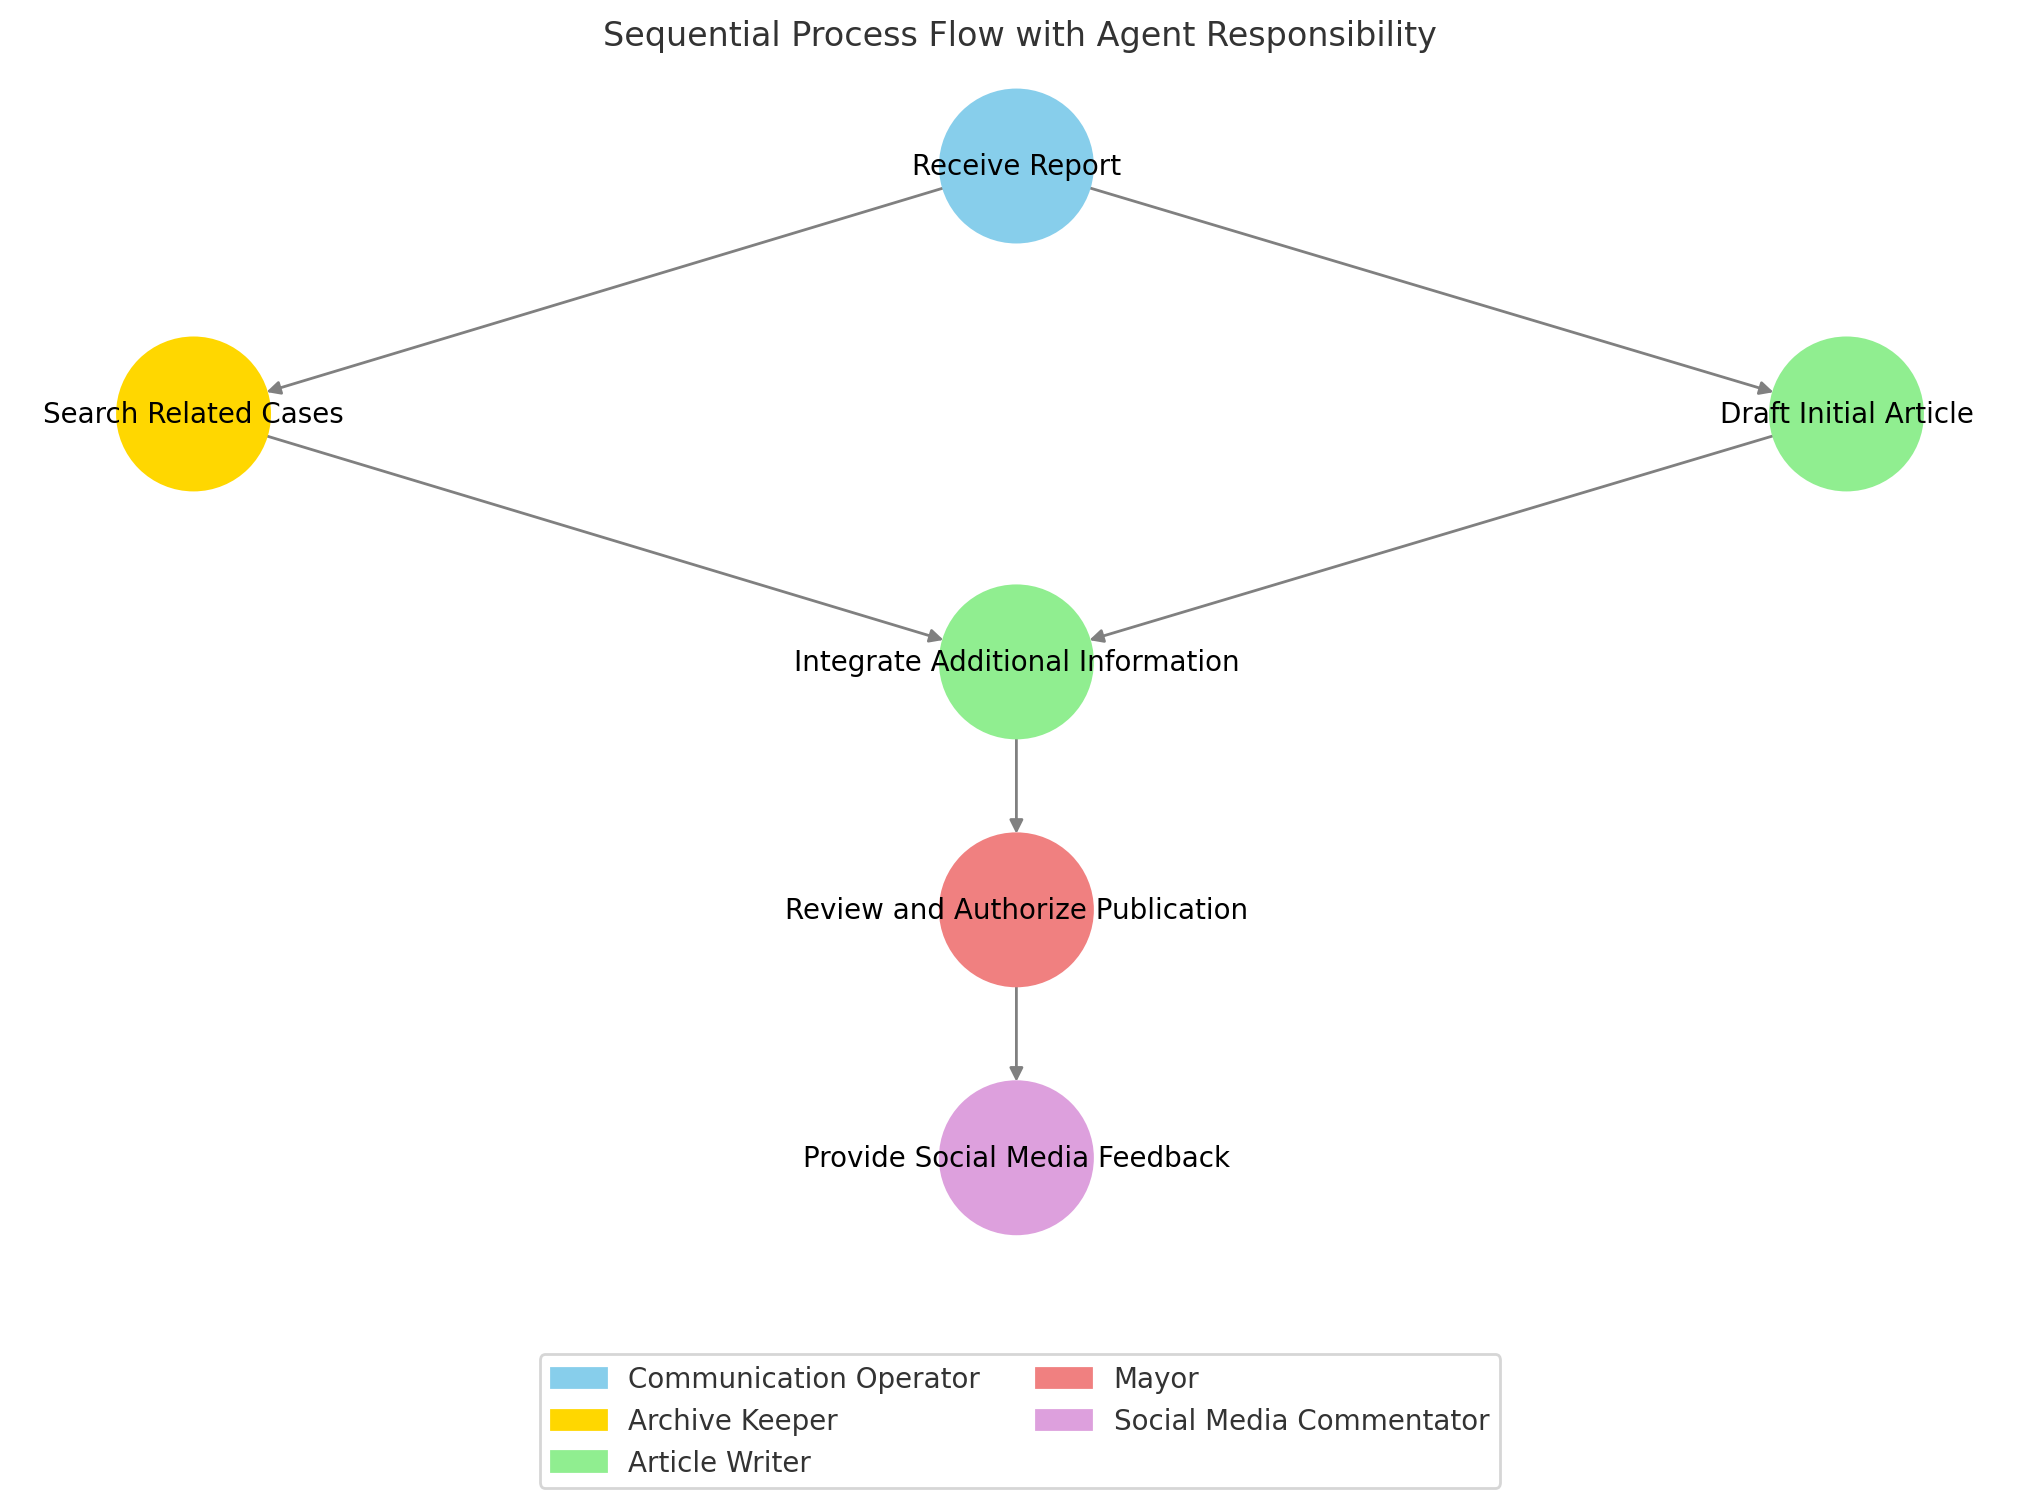
\includegraphics[width=0.9\textwidth]{figures/PC-process.png}
	\caption{Sequential Process Flow of the Medical Services Crew with Agent Responsibilities}
	\label{fig:medical_services_flow}
\end{figure}


\paragraph{Task Dependencies}
The sequential nature of the process requires to establish task dependencies to define the crew's workflow:
\begin{itemize}
	\item \textit{Search Related Cases} and \textit{Draft Initial Article} can be executed in parallel but both depend on \textit{Receive Report}.
	\item \textit{Integrate Additional Information} requires the completion of both \textit{Search Related Cases} and \textit{Draft Initial Article}.
	\item \textit{Review and Authorize Publication} depends on \textit{Integrate Additional Information}.
	\item \textit{Provide Social Media Feedback} requires article approval from the \textit{Mayor}.
\end{itemize}

The task dependencies and agents who perform each task can be observed in Figure~\ref{fig:medical_services_flow}.
